%(BEGIN_QUESTION)
% Copyright 2015, Tony R. Kuphaldt, released under the Creative Commons Attribution License (v 1.0)
% This means you may do almost anything with this work of mine, so long as you give me proper credit

\noindent
{\bf Laboratorieøvelse -- introduksjon}

\vskip 5pt

Oppgaven deres er å bygge, dokumentere og feilsøke et telemetrisystem som består av en analog sensor koblet til en datainnsamlingsmodul (DAQ), som deretter sender data over Ethernet til en PC. Temperatur og trykk er anbefalte prosessvariabler å måle. Elektrisk strøm (målt med shuntmotstand eller strømtransformator) er også en svært god prosessvariabel, og dette fungerer godt som introduksjon til det mer spesialiserte temaet effektmåling og vern. Å sette opp et elektronisk vernerele som måler AC-strøm og sender ``trip''-signal til en bryter, er faktisk et svært godt alternativ til en generisk DAQ. Andre prosessvariabler kan også vurderes.

Tabellen under viser hvilke mål du og teamet ditt må fullføre innen planlagt tid for denne laboratorieøvelsen. Merk at noen mål er individuelle, mens andre gjelder hele teamet:

\underbar{Tabell for måloppnåelse:}

% No blank lines allowed between lines of an \halign structure!
% I use comments (%) instead, so that TeX doesn't choke.

$$\vbox{\offinterlineskip
\halign{\strut
\vrule \quad\hfil # \ \hfil & 
\vrule \quad\hfil # \ \hfil & 
\vrule \quad\hfil # \ \hfil & 
\vrule \quad\hfil # \ \hfil & 
\vrule \quad\hfil # \ \hfil & 
\vrule \quad\hfil # \ \hfil & 
\vrule \quad\hfil # \ \hfil \vrule \cr
\noalign{\hrule}
%
% First row
{\bf Prestasjonsmål} & {\bf Vurdering} & {\bf 1} & {\bf 2} & {\bf 3} & {\bf 4} & {\bf Team} \cr
%
\noalign{\hrule}
%
% Another row
Teammøte og prototypeskisse (gjør dette {\it først!}) & mestring & -- & -- & -- & -- & \cr
%
\noalign{\hrule}
%
% Another row
Konstruksjonsutfordring for krets & mestring & & & & & -- -- -- -- \cr
%
\noalign{\hrule}
%
% Another row
Endelig dokumentasjon og systeminspeksjon & mestring & & & & & -- -- -- -- \cr
%
\noalign{\hrule}
%
% Another row
Demonstrer IP-kommandoen ``ping'' & mestring & -- & -- & -- & -- &  \cr
%
\noalign{\hrule}
%
% Another row
Demonstrer bruk av ``knockout punch''-verktøy & mestring & -- & -- & -- & -- &  \cr
%
\noalign{\hrule}
%
% Another row
Nøyaktig måling av variabel ($\pm$ 1\% av span) & mestring & -- & -- & -- & -- &  \cr
%
\noalign{\hrule}
%
% Another row
Data overført via Ethernet & mestring & -- & -- & -- & -- &  \cr
%
\noalign{\hrule}
%
% Another row
Feilsøking & mestring & & & & & -- -- -- -- \cr
%
\noalign{\hrule}
%
% Another row
Labspørsmål: Instrumenttilkoblinger & proporsjonal &  &  &  &  & -- -- -- -- \cr
%
\noalign{\hrule}
%
% Another row
Labspørsmål: Idriftsetting & proporsjonal &  &  &  &  & -- -- -- -- \cr
%
\noalign{\hrule}
%
% Another row
Labspørsmål: Hoderegning & proporsjonal &  &  &  &  & -- -- -- -- \cr
%
\noalign{\hrule}
%
% Another row
Labspørsmål: Diagnostikk & proporsjonal &  &  &  &  & -- -- -- -- \cr
%
\noalign{\hrule}
%
% Another row
Avvikling og opprydding i lab & mestring & -- & -- & -- & -- &  \cr
%
\noalign{\hrule}
} % End of \halign 
}$$ % End of \vbox

Den eneste ``proporsjonale'' vurderingen i denne aktiviteten er labspørsmålene, som besvares individuelt av hver student. En liste over aktuelle labspørsmål finnes mot slutten av dette arbeidsarket. Spørsmålene skal både styre labarbeidet og måle forståelsen deres, og instruktøren kan derfor stille spørsmålene fortløpende fra dag til dag i stedet for alt på én dag.

\vskip 10pt

{\bf Det er avgjørende at teamet planlegger hva som skal oppnås hver dag. Et kort teammøte (10 minutter) i starten av hver labøkt er en god måte å gjøre dette på: gå gjennom hva som er gjort, hva som gjenstår, og hvilke vurderinger dere må være klare for. Det er mye arbeid i å bygge, dokumentere og feilsøke fungerende instrumentsystemer!}

Etter hvert som dere jobber med systemet, vil dere uunngåelig møte problemer. Forsøk alltid å løse disse som team før dere ber instruktøren om hjelp. Hvis dere fortsatt trenger hjelp, skriv teamfargen deres på labtavla sammen med en kort beskrivelse av hva dere trenger hjelp til. Instruktøren følger opp teamene i den rekkefølgen de står på tavla.




\vfil \eject

\noindent
{\bf Laboratorieøvelse -- teammøte, prototypeskisse og valg av instrumenter}

\vskip 5pt

Et viktig første steg i denne laboratorieøvelsen er å {\bf møte instruktøren} som team for å diskutere sikkerhet, samarbeid og konkrete roller i teamet. Hvis dere vil prioritere erfaring med bestemt utstyr (for eksempel en bestemt type styringssystem eller bestemte verktøy), teknikker (for eksempel mekanisk bearbeiding), eller oppgaver for å styrke ferdigheter, er dette tidspunktet å ta det opp slik at læringsutbyttet blir størst mulig.

\vskip 10pt

Et helt nødvendig steg er å jobbe sammen om å {\bf lage en prototypeskisse} av systemet dere planlegger å bygge. Vanligvis er dette et enkelt elektrisk skjema og/eller sløyfediagram som viser alle elektriske forbindelser mellom komponenter, samt eventuell tubing eller rørføring for fluid. Skissen trenger ikke være komplett ned til minste detalj, men må være detaljert nok til at instruktøren kan vurdere om alle komponenter blir korrekt koblet for sikker drift.

For eksempel: hvis dere skal koble feltutstyr til en PLC (Programmable Logic Controller), må skissen vise hvordan utstyret kobles til typiske inn-/utgangsterminaler på PLC, hvor strømforsyning kommer inn, osv. Skissen trenger ikke vise alle mellomkoblinger, for eksempel rekkeklemmer i koblingsbokser mellom feltinstrument og kontroller.

Bruk gode problemløsningsmetoder når dere lager skissen: slå opp i manualer, marker strømretninger, spenningspolaritet og identifiser kilder/laster. Bruk dette som trening i analytisk arbeid. Husk at dere i programmet også vil bli utfordret til å gjøre dette selvstendig (i ``capstone''-vurderinger). Ikke gjør feilen å lene dere på lagkamerater for å løse alt; jobb som om det er en oppgave {\it du} må kunne løse, og sammenlign så resultatene i teamet.

Prototypeskissen er så viktig at instruktøren krever at planen foreligger før bygging starter. {\it Team som bygger uten godkjent plan, vil bli stoppet og får ikke fortsette før plan er utarbeidet og godkjent!} Dere skal heller ikke avvike fra prototype uten godkjenning, for å unngå skade på utstyr ved feil koblinger. Hvert teammedlem bør ha enkel tilgang til planen (helst egen kopi) gjennom hele byggeprosessen. Å skissere før bygging er en ferdighet og vane dere bør ta med dere videre i yrket.

\vskip 10pt

Hvert teamskap i laben har egen DAQ-enhet, og flere DAQ-er kan lånes av instruktør. Dere må installere programvare på en PC for å kunne hente inn analoge data fra DAQ.

Det anbefales å teste DAQ før den kobles til ekstern krets. For enkel test av analog inngang: sett multimeteret i ``Diode Test'' slik at det gir ut en liten spenning, og koble måleledningene til en analog inngangskanal på DAQ. Programvaren skal da vise en liten spenning på kanalen, som bekrefter at DAQ fungerer.

\vskip 10pt

Dere må velge en passende sensor til en av de analoge DAQ-inngangene. For best nøyaktighet anbefales en standard 4--20 mA sløyfedrevet trykk- eller temperaturtransmitter, med 250 ohm motstand mot DAQ slik at DAQ leser et 1--5 V-signal:

$$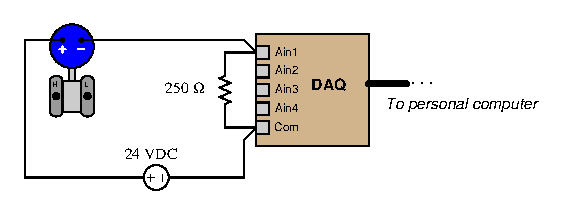
\includegraphics[width=15.5cm]{i00350x01.eps}$$

\filbreak

Dere kan også være mer kreative og bygge en enklere analog målekrets, som denne:

$$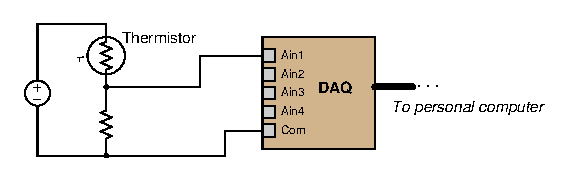
\includegraphics[width=15.5cm]{i00350x02.eps}$$

Utfordringen med en slik krets er at den {\it ikke} gir et lineært signal proporsjonalt med temperatur slik sløyfedrevet transmitter gjør. For å få dette til å fungere, må dere programmere en formel i DAQ-programvaren som ``lineariserer'' spenningen til en proporsjonal temperaturverdi. Dette krever ekstra arbeid: karakteriser sensoren og utvikle en formel som beskriver signalspenning som funksjon av målevariabelen. Et regneark kan være nyttig her: plott kurve for spenning mot stimuli (f.eks. temperatur), og bruk kurvetilpasning for å finne en ligning.

$$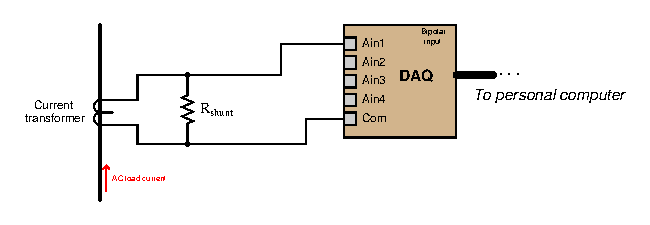
\includegraphics[width=15.5cm]{i00350x05.eps}$$

Hvis dere velger å måle AC-strøm med strømtransformator (CT, vist over), må dere velge en passende shuntmotstand for spenningsfallet fra CT-strømmen. Dette gjøres ved å slå opp CT-ens ``burden''-rating, som angir hvor stor lastmotstanden kan være. CT-er oppfører seg som strømkilder og ``ønsker'' derfor lav lastmotstand (for eksempel et amperemeter). Samtidig må DAQ se stort nok spenningsfall over shunten for å bruke en fornuftig del av måleområdet, slik at oppløsningen utnyttes. {\it Hvis dere bygger denne kretsen, må dere sikre at CT-sekundæren aldri blir åpen når laststrøm går gjennom! Åpen sekundær på strømtransformator kan gi farlig høy spenning!!!}

\vskip 10pt

{\bf Planlegging av et fungerende system bør ikke ta mer enn én time når teamet jobber effektivt, og kan spare dere for mange timer frustrasjon (og mulig ødeleggelse av komponenter)!}




\vfil \eject

\noindent
{\bf Laboratorieøvelse -- utfordring i kretsdesign}

\vskip 5pt

Bygg en enkel krets med enten lyssensor (fotocelle) eller temperatursensor (termistor), koblet med fast motstand og batteri slik at kretsen gir variabel utgangsspenning når sensoren påvirkes. Kretsen skal enten gi økende voltmeterverdi ved økende stimuli (mer lys/varme gir mer spenning -- direkte virkning), eller det motsatte (revers virkning), slik instruktøren angir. Alle elektriske koblinger skal lages med rekkeklemme (ingen tvinnede ledninger, skjøtehylser, wire nuts, fjærklemmer eller krokodilleklemmer). Dere må også vise hvordan dere registrerer og viser laveste og høyeste spenning fra kretsen ved å bruke ``min/max''-funksjonen på multimeteret.

Øvelsen tester evnen til å identifisere sensorens virkemåte, dimensjonere motstand for spenningsdeler med sensoren, koble voltmeteret slik at responsretningen blir riktig, bruke DMM til å fange min-/maksverdier, og bruke rekkeklemme for ryddige og sikre koblinger.

$$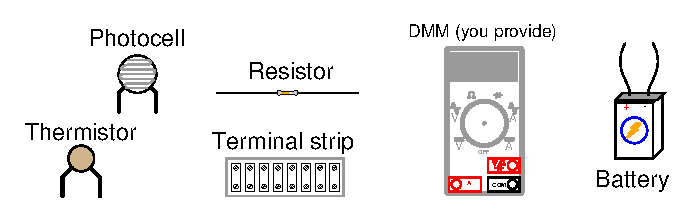
\includegraphics[width=15.5cm]{i00350x06.eps}$$

\vskip 10pt

Følgende komponenter/materialer er tilgjengelige: ulike CdS-{\bf fotoceller} og {\bf termistorer}; assorterte {\bf motstander}; {\bf rekkeklemmer}; lengder med {\bf koblingsledning}; {\bf batteriklemmer} (holdere).

\vskip 10pt

Dere må selv stille med skrutrekkere og digitalt multimeter (DMM) for montering og test ved pulten. Instruktøren leverer batteri(er) når dere er klare til funksjonstest. Frem til da skal kretsen være spenningsløs.

\vskip 10pt

\noindent
{\bf Meterrespons} (instruktør velger): \hskip 20pt \underbar{\hskip 20pt} Direkte \hskip 20pt \underbar{\hskip 20pt} Revers

\vskip 10pt

\noindent
{\bf Fanget verdi} (instruktør velger): \hskip 20pt \underbar{\hskip 20pt} $V_{minimum}$ \hskip 20pt \underbar{\hskip 20pt} $V_{maximum}$

\vskip 10pt

\noindent
{\bf Sensortype} (instruktør velger): \hskip 20pt \underbar{\hskip 20pt} Fotocelle \hskip 20pt \underbar{\hskip 20pt} Termistor






\vfil \eject

\noindent
{\bf Laboratorieøvelse -- bygging av systemet}

\vskip 5pt

Instrumenteringslabben er rigget for bygging av fungerende instrumentsløyfer, med over et dusin koblingsbokser, ferdigtrukne signalkabler og ``racks'' med 2-tommers vertikale rør for instrumentmontering. De eneste ledningene dere normalt trenger å legge, er fra feltinstrument til nærmeste koblingsboks, samt korte ``jumper''-kabler mellom ferdiginstallerte kabler i mellomliggende koblingsbokser.

Etter at prototypeskissen er godkjent av instruktør, kan dere starte bygging. Alle ledningsforbindelser skal gjøres med rekkeklemmer. Tvinnede eller teipede skjøter tillates ikke.

\vskip 10pt

Dere må konfigurere DAQ-programvaren til å ``skalere'' 1--5 VDC-signalet til faktisk måleverdi for prosessvariabelen (f.eks. temperatur, trykk). Det er et krav at DAQ viser prosessvariabelen dere måler, ikke bare rå signalspenning.

\vskip 10pt

PC-en koblet til DAQ kan være egen laptop eller en av lab-PC-ene. Uansett hvilken PC dere bruker, må den kobles til labens Ethernet-nettverk slik at en annen PC i laben kan hente data fra den.

\vskip 10pt

Det valgte systemet kan kreve eget kapslingsskap for DAQ og/eller andre komponenter som ikke allerede inngår i labens faste sløyfesystem. Hvis dere må lage hull i et skap, skal dere bruke et spesialverktøy kalt {\it knockout punch} (ikke hullsag i drill). Greenlee lager en serie slike verktøy kalt {\it Slug Buster}, som det kan være lurt å sette seg inn i før bruk.

\vskip 10pt

{\bf Vanlige feil:}

\begin{itemize}
\item{} Starte bygging før kretsen er planlagt på papir med foreslått skisse.
\item{} Ikke ta hensyn til spenningsgrenser på DAQ-ens analoge innganger. {\it Pass på å ikke overbelaste DAQ med signalspenninger over målegrensene!}
\item{} Ikke dra i hver enkelt leder ved terminering for å kontrollere mekanisk god forbindelse.
\item{} Studenter jobber isolert på hver sin del og deler ikke med teamet hva de har gjort og hvordan. Hele teamet må lære hele systemet.
\end{itemize}

\vskip 10pt

{\bf Bygging av et fungerende system bør ikke ta mer enn én full labøkt (3 timer) dersom komponenter er tilgjengelige og teamet jobber effektivt!}





\vfil \eject

\noindent
{\bf Laboratorieøvelse -- avansert bruk av multimeter}

\vskip 5pt

En del av øvelsen er å lære en svært kraftig funksjon i digitalmultimeteret: evnen til å fange og lagre minimums- og maksimumsverdier. På Fluke-målere aktiveres dette med knapp merket ``Min/Max''. Når modusen er aktiv, lagrer måleren laveste, høyeste og gjennomsnittsverdi fra aktiveringstidspunktet frem til du leser av de lagrede verdiene.

Noen DMM-er har enda mer avanserte funksjoner, der flere datapunkter logges over tid, mer som en datalogger. Fluke-målere tilbyr også funksjoner som {\it high-speed Min/Max}, {\it high-resolution measurement} og {\it low-pass filtering}. Bruk tid på å prøve disse funksjonene i løpet av øvelsen.

\vskip 10pt

Funksjonene er viktige ved feilsøking av intermittente feil. Når multimeteret kan fange og lagre måleverdier over tid, kan teknikeren bruke måleren som registreringsenhet, gjøre andre oppgaver, og senere komme tilbake for å se hva som ble registrert.

\vskip 10pt

Merk at multimeteret kanskje ikke beholder autoranging i registreringsmodus. Hvis måleverdien er lav ved oppstart av registrering, kan måleren vise ``overload'' dersom signalet senere overstiger låst område. I så fall bør du sette måleområdet manuelt før du aktiverer registrering.

Noen DMM-er tilbyr også flere samplingshastigheter i loggfunksjonen, for eksempel ``slow'' og ``fast''. Raskere sampling gir, som ellers i DAQ, lavere oppløsning. Du kan dermed få mindre presisjon ved høy hastighet. Ønsker du maksimal oppløsning, må du ofte akseptere lavere samplingshastighet.

\vskip 10pt

{\bf Vanlige feil:}

\begin{itemize}
\item{} Ikke lese brukermanualen for multimeteret.
\item{} Ikke lese brukermanualen for multimeteret.
\item{} Ikke lese brukermanualen for multimeteret.
\item{} Merk: {\it denne gjentakelsen er ikke en skrivefeil. Jeg vil {\bf virkelig} at du leser manualen som fulgte med multimeteret!}
\end{itemize}




\vfil \eject

\noindent
{\bf Laboratorieøvelse -- dokumentasjon av systemet}

\vskip 5pt

Hver student skal lage sin egen {\it systemskisse} for teamets datainnsamlingssystem. Dette blir ikke et ISA-standard sløyfediagram, men en kombinasjon av skjema (sensor- og DAQ-koblinger) og blokkskjema (PC-nettverk over Ethernet med IP-adresser). Diagrammet må være {\it komplett} og {\it detaljert}, og vise alle ledningskoblinger, alle kabler, alle rekkeklemmer, måleområder, nettverksadresser osv.

Eksempel på systemdiagram:

$$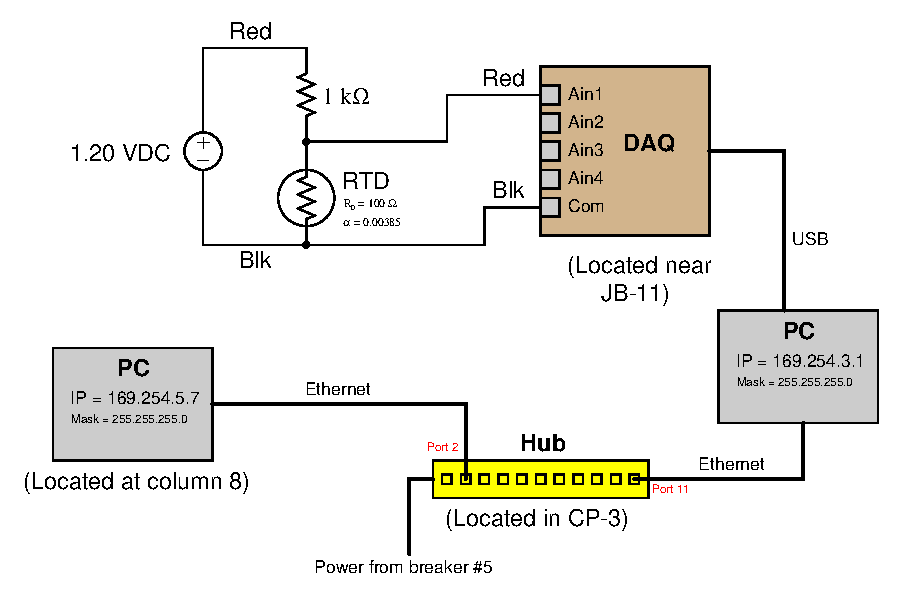
\includegraphics[width=15.5cm]{i00350x03.eps}$$

Når hele teamet er ferdig med individuelle diagrammer, tilkalles instruktør for systeminspeksjon. Da går studentene gjennom systemet på omgang, mens de andre kontrollerer diagrammene sine for feil og mangler. Instruktøren kontrollerer også installasjonskvalitet: frynsete ledere, dårlig crimpejobbing, dårlig kabelføring, manglende merking, manglende wire-duct-lokk osv. Teamet må rette alle avvik for å få godkjent systemet.

Etter godkjent inspeksjon skal hvert teammedlem legge systemdiagrammet i diagramholderen midt i laben bak hovedpanelet. Når dere senere skal feilsøke et annet teams system, er dette stedet dere finner diagrammet.

\vskip 10pt

{\bf Vanlige feil:}

\begin{itemize}
\item{} Glemme merking av alle signalledere.
\item{} Glemme å notere alle lederfarger.
\item{} Glemme navn på diagrammet.
\item{} Basere eget diagram på en lagkamerats diagram i stedet for å kontrollere systemet selv.
\item{} Ikke plassere instrumenter i riktig orientering (feltinstrumenter til venstre, kontrollromsinstrumenter til høyre).
\end{itemize}



\vfil \eject

\noindent
{\bf Laboratorieøvelse -- signal skalering/linearisering i DAQ}

\vskip 5pt

Hvert team skal konfigurere DAQ-systemet slik at det måler og rapporterer prosessvariabelen korrekt. Nøyaktigheten kontrolleres av instruktør ved å påføre tilfeldige stimuli på sensoren mens teamet verifiserer fjernvisningen (på PC koblet via nettverk til DAQ-modulen).

Hvis systemet bruker sløyfedrevet 4--20 mA-transmitter, trenger dere normalt kun å ``skalere'' DAQ slik at lineært 1--5 VDC-signal konverteres til lineær representasjon av målevariabelen. Dere må imidlertid støtte dere på teammedlemmer som har tatt INST24X-kursene for å kalibrere transmitteren slik at den faktisk leverer korrekt 4--20 mA-signal.

Hvis systemet leser råspenning fra en resistiv sensor i bro- eller annen spenningsdelerkobling, må DAQ-programvaren settes opp til å ``linearisere'' signalet slik at den viser faktisk prosessvariabel og ikke kun spenning. Skjermbildet under viser hvordan regneark kan brukes til å generere en lineariseringsligning fra publiserte sensordata:

$$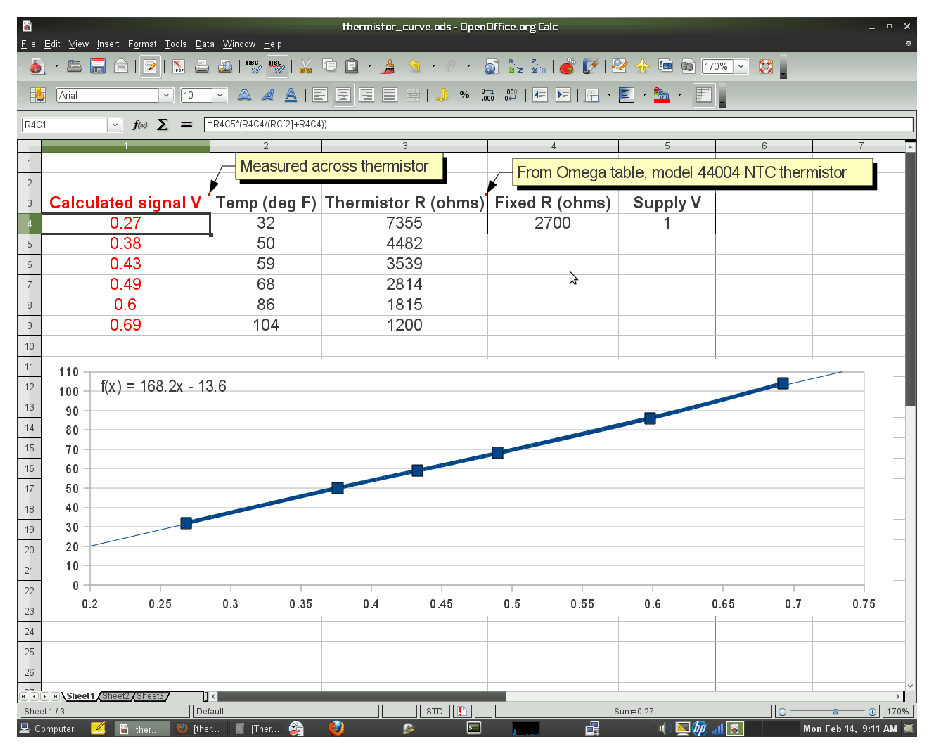
\includegraphics[width=15.5cm]{i00350x04.eps}$$

I dette eksemplet er sensoren en NTC-termistor (negative temperature coefficient), modell 44004 fra Omega. Formelen i cellene R4C1 til R9C1 beregner spenningsfallet over en fast motstand (2700 $\Omega$) i serie med termistoren ved 1 V DC-kilde, med spenningsdelerformelen ($V_R = V_{source} {R \over {R_{total}}}$). Termistorverdiene i kolonne 3 er hentet fra Omegas tabell for modell 44004. Et ``scatter''-plott viser temperatur som funksjon av spenning, og en ``trendline'' brukes til å tilpasse datapunktene til en matematisk ligning. I dette tilfellet ble ligningen Temp = 168.2 * (Voltage) $-$ 13.6. Denne må legges inn i DAQ-programvaren, slik at målt spenning oversettes til temperatur.

\filbreak

Hvis sensoren dere velger ikke har datatabell, kan dere lage en egen ved å utsette sensoren for kjente stimuli og måle motstand ved disse verdiene. Deretter kan regneark brukes til å plotte spenningsrespons og utlede en ligning.

En stor fordel med regnearkmodellering av signalspenning mot temperatur er at dere kan ``eksperimentere'' med ulike faste motstandsverdier for å se effekten på linearitet. Endres fast motstand i regnearket, ser dere umiddelbart hvordan kurven endres, og hvordan signalstyrken påvirkes.

\vskip 10pt

{\bf Vanlige feil:}

\begin{itemize}
\item{} Velge kalibreringsreferanse med for dårlig nøyaktighet (f.eks. kalibrere Rosemount-transmitter til $\pm$ 0.1 PSI med et billig manometer som kun leser nærmeste 5 PSI).
\item{} Feil oppsett av scatter-plott i regneark ved ligningstilpasning (f.eks. variabler på feil akser).
\end{itemize}

\vskip 10pt

{\bf Sensor-karakterisering og DAQ-skalering bør ikke ta mer enn én full labøkt (3 timer) hvis teamet jobber effektivt!}




\vfil \eject

\noindent
{\bf Laboratorieøvelse -- dataoverføring over Ethernet}

\vskip 5pt

En viktig del av øvelsen er at innsamlede data transporteres over Ethernet. Med mindre DAQ-programvaren er avansert, er dette ofte ikke direkte støttet. Et godt alternativ er at én PC samler data fra DAQ, mens en annen PC viser skjermbildet til den første via fjernaksess. Dette kan gjøres med ``Remote Desktop'' i Microsoft Windows, eller gratis fjernstyringsprogram som {\tt RealVNC}.

Fjernaksess gjør ikke bare at dere ser live data fra DAQ over nettverket, men lar dere også {\it styre} DAQ-PC-en eksternt. Å kunne bruke slik programvare er derfor en nyttig ferdighet.

\vskip 10pt

Et annet Ethernet-mål i øvelsen er bruk av {\tt ping}-kommandoen for nettverkstest. Når to PC-er er korrekt koblet til samme Ethernet-nett, skal dere kunne ``pinge'' den ene fra den andre ved å bruke IP-adressen som argument til {\tt ping}. Kommandoen kjøres i kommandolinjevindu i Windows. Flere detaljer finnes i læreboka {\it Lessons In Industrial Instrumentation}.

En vellykket ``ping'' er en {\it nødvendig} betingelse for fjernvisning, men ikke en {\it tilstrekkelig} betingelse. En PC som ikke svarer på ping, er definitivt ikke klar for fjerninnlogging. En PC som svarer på ping, er heller ikke nødvendigvis helt klar for fjerninnlogging. Ping er bare første steg i full kommunikasjon.

\vskip 10pt

Hvis ping mislykkes, er noe i kommunikasjonen mellom enheten og PC-en som pinger blokkert. Et godt neste steg er å pinge andre enheter i samme nett. Lykkede ping-forsøk beviser at OSI-lag 1, 2 og 3 fungerer mellom disse punktene, siden ping krever disse lagene. Når dere vet hvilke nettverksdeler som fungerer, kan dere snevre inn feilmulighetene.

\vskip 10pt

Funksjoner over OSI-lag 3 (for eksempel brannmurprogramvare på PC-er) kan blokkere kommunikasjon i labnettet, inkludert ping. Hvis dere bruker egen laptop i labnettet, kan det være enklere midlertidig å deaktivere sikkerhetsfunksjoner for å åpne kommunikasjon med øvrige enheter. Husk å aktivere sikkerhetsfunksjonene igjen når dere er ferdige, slik at PC-en ikke er ubeskyttet neste gang den kobles til Internett.



\vfil \eject

\noindent
{\bf Laboratorieøvelse -- feilsøking}

\vskip 5pt

Den mest krevende delen av øvelsen er {\it feilsøking}, der du viser at du kan isolere feil i systemet med logisk metode. All feilsøking vurderes individuelt (ingen teampoeng), og skal gjøres {\it på et system du ikke har vært med å bygge}, slik at du må bruke sløyfediagrammer aktivt i stedet for hukommelse fra byggingen.

Hver student får begrenset tid til å identifisere både generell plassering og type feil, samt logisk begrunne diagnostiske steg. All feilsøking skjer under direkte oppsyn av instruktør for å sikre selvstendig og effektiv gjennomføring.

Hvis du ikke identifiserer både feilplassering og feiltype innen tidsfristen, og/eller ikke viser rasjonell diagnostisk metode, blir forsøket underkjent. Da må studenten prøve på nytt med en annen feil. Flere nye forsøk er tillatt uten trekk i karakter.

Kun standard multimeter er tillatt testutstyr innen tidsfristen. Brudd i krets for testing er ikke tillatt uten instruktørens tillatelse, og da bare etter korrekt forklaring av hvilke problemer et slikt inngrep kan skape i et reelt anlegg.

Instruktøren går gjennom hvert feilsøkingsforsøk i etterkant og peker på gode og svake punkter. Feilsøking er en ferdighet som bygges gjennom øvelse og feil, så ikke bli motløs hvis du trenger flere forsøk. En viktig livslære i denne aktiviteten er å håndtere nederlag, fordi det {\it vil} skje i arbeidslivet. Det er ingen skam å ikke lykkes på første forsøk når du har gjort et seriøst arbeid. Det som ikke er akseptabelt, er snarveier eller å gi opp.

\vskip 10pt

{\bf Vanlige feil:}

\begin{itemize}
\item{} Unnlate å ta målinger med multimeter.
\item{} Unnlate å kontrollere andre relevante målinger i systemet (f.eks. manometeravlesninger).
\item{} Feiltolke diagrammet (f.eks. tro at du står på feil sted i systemet under måling).
\item{} Feil bruk av multimeter (f.eks. AC i stedet for DC, feil område, feil plassering av måleledninger). Dette skjer ofte når student møter uforberedt og må låne et annet instrument enn sitt eget.
\end{itemize}

\vskip 10pt

{\bf Husk at hensikten med feilsøkingsøvelsen er å utvikle og vurdere evnen til intelligent diagnose av komplekse systemer. Å finne feilen ved flaks eller ren prøve-og-feile-kontroll er ikke en godkjent ferdighetsdemonstrasjon. Det som teller, er dokumentert evne til logisk analyse og isolering av problemet, med riktig forklaring av alle steg!}

\vskip 10pt

{\bf Feilsøking krever mye labtid, ofte minst to 3-timers økter for at en full klasse skal komme i mål. Teamet må budsjettere tid til dette i planen, og dere bør benytte muligheten til å observere andre under feilsøking for å lære metoden bedre.}



\vfil \eject

\noindent
{\bf Labspørsmål}

\vskip 5pt

\begin{itemize}
\item{} {\bf Instrumenttilkoblinger}
\item{} Bestem riktige lederkoblinger mellom DAQ-modul og elektrisk sensor, basert på diagrammer med merkede terminaler
\item{} Identifiser korrekt alle elektriske kilder/laster, samt spenningspolaritet og strømretning i DAQ/sensorkrets, basert på diagrammer med merkede terminaler
\end{itemize}

\filbreak

\begin{itemize}
\item{} {\bf Idriftsetting og dokumentasjon}
\item{} Forklar virkemåten til sensoren brukt i systemet
\item{} Forklar forskjellen mellom {\it single-ended} inngang og {\it differential} inngang på en analog DAQ-modul
\item{} Beskriv noen avanserte funksjoner i multimeteret {\it utover} loggmodus (``Min/Max'')
\item{} Forklar hvorfor kraft- og signalkabling ikke bør føres sammen i samme rør eller panel
\item{} Forklar hvorfor det er nødvendig med {\it bushing} for å beskytte ledninger som går inn/ut av kapsling gjennom hull i sideveggen
\end{itemize}

\filbreak

\begin{itemize}
\item{} {\bf Hoderegning} (kalkulator ikke tillatt!)
\item{} Finn tillatt kalibreringsfeil for instrument (f.eks. +/- 0.5\% for instrument med område 200 til 500 grader)
\item{} Konverter 1--5 V-signal til prosent av span (f.eks. 3.5 V = \underbar{\hskip 20pt}\%)
\item{} Konverter prosent av span til 1--5 V-signal (f.eks. 70\% = \underbar{\hskip 20pt} V)
\item{} Beregn ADC-oppløsning gitt antall bit og inngangsområde
\end{itemize}

\filbreak

\begin{itemize}
\item{} {\bf Diagnostikk}
\item{} Forklar hvordan man skiller kabelbrudd (``open'') fra kortsluttet kabel (``short'') med kun voltmeter (ingen strøm- eller motstandsmåling, men anta at kretsen kan brytes for test)
\item{} Vurder om en gitt diagnostisk test gir nyttig informasjon ut fra et sett symptomer i et feilet system
\item{} Identifiser minst to plausible feil gitt resultat av en diagnostisk test og et symptomsett fra et feilet system
\item{} Foreslå en diagnostisk test for et feilet system og forklar betydningen av to ulike mulige testresultater
\end{itemize}



\vfil \eject

\noindent
{\bf Laboratorieøvelse -- avvikling og opprydding}

\vskip 5pt

Siste steg i øvelsen er å avvikle hele teamets system og tilbakeføre utvalgte komponenter til riktig lagerplass, slik at laben klargjøres for neste øvelse. Ta ned systemdokumentasjon (f.eks. sløyfediagram) fra felles oppbevaringsområde og kast eller behold for egne notater. Fjern også instrumentmerker (f.eks. FT-101) fra instrumenter og kabler. Utfør generell opprydding: kast avfall, legg verktøy tilbake på riktig plass, rydd bort ledningsrester fra gulv og koblingsbokser osv.

\vskip 10pt

\indent
{\bf La følgende komponenter stå montert på rackene:}

\begin{itemize}
\item{} Store reguleringsventiler og posisjonere
\item{} I/P-omformere
\item{} Store elektriske motorer
\item{} Store frekvensomformere (VFD)
\item{} Kabler i rør mellom koblingsbokser
\item{} Rør- og tubefittings (ikke skru opp gjengede rørkoblinger)
\item{} Forsyningsregulatorer for instrumentluft
\end{itemize}

\vskip 10pt

\indent
{\bf Returner følgende komponenter til riktig lagringsplass:}

\begin{itemize}
\item{} Følerelementer (f.eks. termoelementer, pH-prober, osv.)
\item{} Prosess-transmittere
\item{} ``Jumper''-kabler brukt mellom rekkeklemmer i samme koblingsboks
\item{} Plasttubing og tube-fittings (kobles fra kompresjonsfittings)
\item{} Strømkabler og skjøteledninger
\item{} Justerbare lufttrykksregulatorer (loading-station)
\end{itemize}

\vskip 10pt

Til slutt skal alle komponenter i styringssystemet tilbakeføres til original standardkonfigurasjon (fabrikkstandard). Dette inkluderer PID-innstillinger, funksjonsblokkprogram, inngangsområder osv.


\underbar{file i00350}
%(END_QUESTION)





%(BEGIN_ANSWER)

Det finnes rimelige datainnsamlingsmoduler for PC på markedet, inkludert noen med USB-grensesnitt (og mange med RS-232 seriellgrensesnitt). Har du kun seriellmodul og en PC med bare USB (som de fleste laptoper), kan du bruke en USB-til-seriell-adapter for å koble DAQ-enheten til PC. I Microsoft Windows kan du sette opp operativsystemet slik at USB-adapteren vises som eldre COM1/COM2-seriellport. Da vil DAQ-programvaren normalt kommunisere sømløst med DAQ-modulen via adapteren.

%(END_ANSWER)





%(BEGIN_NOTES)

\noindent
{\bf Diagrammer / inspeksjon:}

Jeg anbefaler sterkt å krysse av studentenes diagrammer mens systemet inspiseres (sikker terminering, korrekt tubing, god føringsvei osv.). La alle teammedlemmer ta deg med på en ``omvisning'' av systemet, der hver student forklarer en valgt del ved hjelp av sitt eget diagram. Mens én student forklarer, kan du kontrollere de andres diagrammer for korrekthet. Dette sparer tid ved å kombinere inspeksjon og diagramkontroll, og sikrer at studentene faktisk kan knytte diagrammet til det de har bygget og formidle forståelsen.

\vskip 10pt

\goodbreak

\noindent
{\bf Forslag til feilsøkingsfeil:}

\begin{itemize}
\goodbreak
\item{} Avisoler leder ved terminal, men klem fast isolert del i stedet for blank leder (lederbrudd)
\item{} Kutt signalkabel et sted i rørføring (lederbrudd)
\item{} Koble fra Ethernet-kabel
\item{} Endre IP-adresse eller nettmaske på én PC
\item{} Koble lederne i instrumentkabel omvendt (byggefeil)
\item{} Sett transmitter med for høy demping (treg respons)
\item{} Sett indikator/regulator med for høy demping (treg respons)
\item{} Feilkalibrer transmitter og/eller indikator/regulator (unøyaktighet)
\item{} Tett tubeforbindelse med bit av skumørepropp i fittings (treg respons)
\item{} Feilkonfigurer linearisering i transmitter og/eller DAQ (ikke-linearitet)
\item{} Feilkonfigurer funksjonsblokk i DAQ (f.eks. grenseverdier slik signal låser lav/høy; bryt signallinje mellom blokker)
\item{} Koble 2.2 k motstand parallelt med 4--20 mA-transmitter for å simulere delvis kortslutning i kabling (unøyaktighet)
\item{} Bytt 250 ohm motstand med annen som ser lik ut, men har feil verdi (unøyaktighet)
\item{} Del ut feil diagram til studentene (dokumentasjonsfeil)
\end{itemize}













\vfil \eject

\noindent
{\bf Labspørsmål}

\vskip 20pt

\begin{itemize}
\item{$(1)$} Koble transmitteren slik at trykk registreres på kanal 3 i DAQ:

$$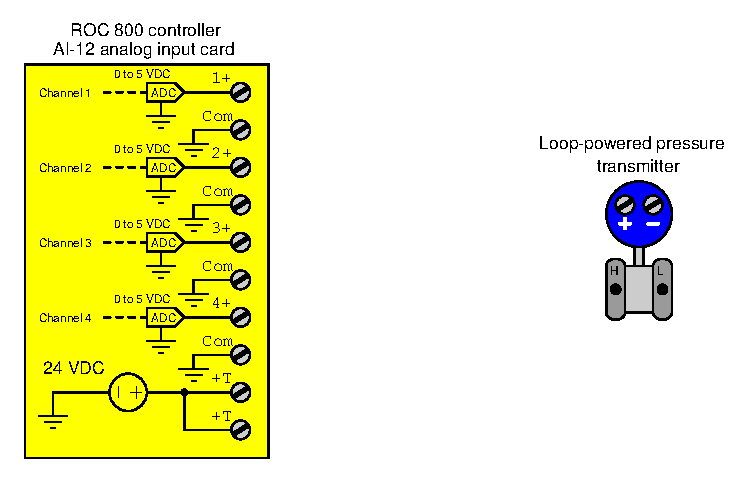
\includegraphics[width=15.5cm]{i00350x07.eps}$$

\vskip 20pt

\item{$(2)$} Forklar forskjellen mellom {\it single-ended} og {\it differential} innganger på en analog DAQ-modul.

\vskip 20pt

\item{$(3)$} Bestem tillatt kalibreringsfeil for en trykktransmitter med område 0 til 300 PSI og kalibreringstoleranse $\pm$ 0.5\%. Oppgi svaret i PSI.

\vskip 20pt

\item{$(4)$} PC nummer 3 (IP-adresse 192.168.0.2) får ikke kontakt med internett. Angi én diagnostisk test du kan gjøre, og beskriv {\it to ulike mulige resultater} av testen. Forklar hva hvert resultat betyr for lokalisering av feilen:

$$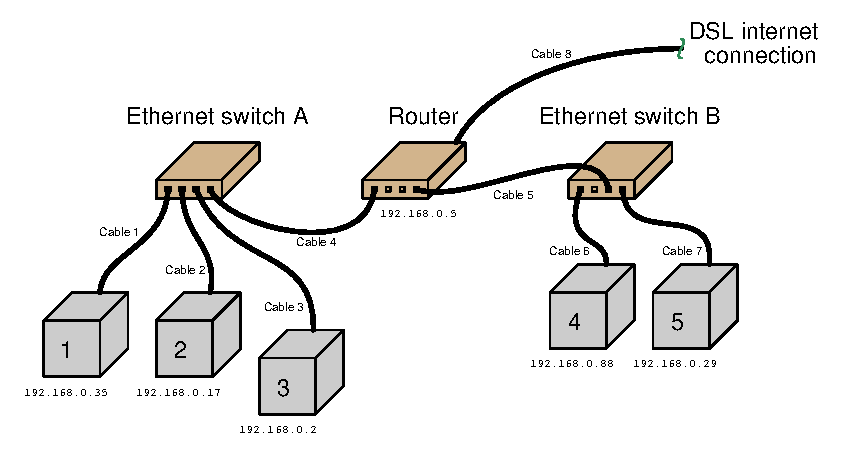
\includegraphics[width=15.5cm]{i00350x09.eps}$$
\end{itemize}












\vfil \eject

\noindent
{\bf Labspørsmål}

\vskip 20pt

\begin{itemize}
\item{$(1)$} Koble transmitteren slik at trykk registreres på kanal 2 i DAQ:

$$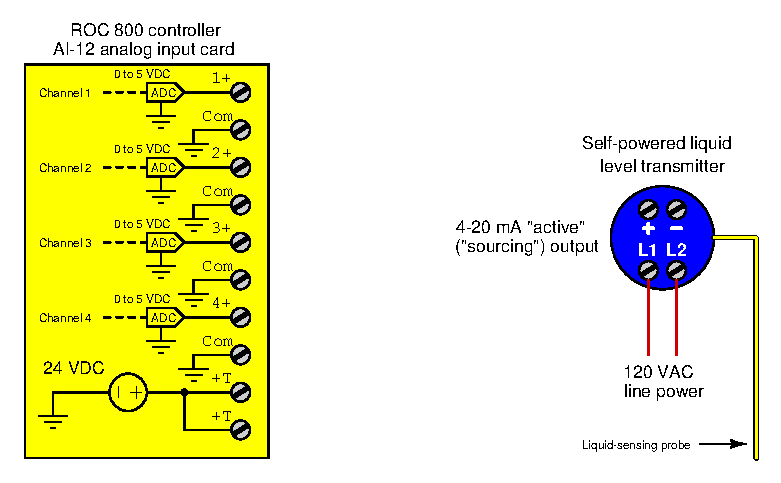
\includegraphics[width=15.5cm]{i00350x08.eps}$$

\vskip 20pt

\item{$(2)$} Nevn minst én avansert funksjon i multimeteret {\it utover} loggmodus (``Min/Max'').

\vskip 20pt

\item{$(3)$} Konverter et 2.5 volts signal (innenfor 1--5 volt område) til verdi uttrykt i {\it prosent}.

\vskip 20pt

\item{$(4)$} PC nummer 5 (IP-adresse 192.168.0.29) får ikke kontakt med PC nummer 1 (IP-adresse 192.168.0.35). Angi én diagnostisk test du kan gjøre, og beskriv {\it to ulike mulige resultater} av testen. Forklar hva hvert resultat betyr for lokalisering av feilen:

$$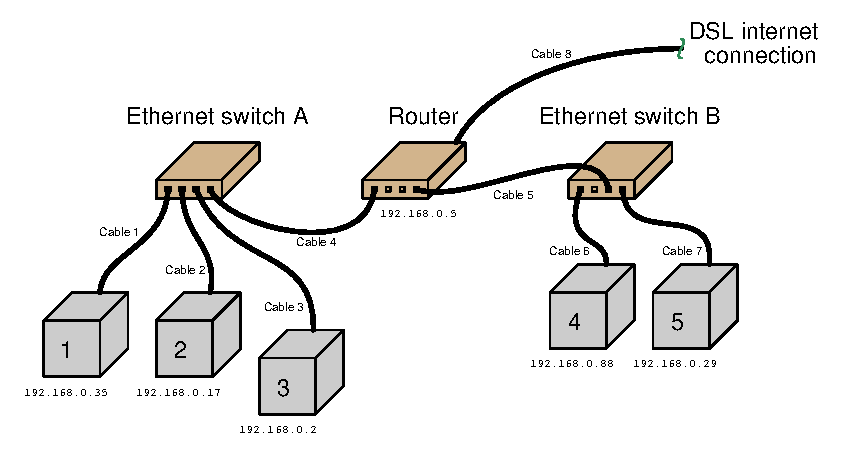
\includegraphics[width=15.5cm]{i00350x09.eps}$$
\end{itemize}


%INDEX% Lab exercise, data acquisition and Ethernet networking

%(END_NOTES)
